\documentclass[a4paper,kulak]{kulakarticle}

\usepackage[utf8]{inputenc}
\usepackage[dutch]{babel}
\usepackage{pdfpages}
\usepackage{subfig}
\usepackage{float}

\usepackage{cite}

% style
%\usepackage[left=2.5cm,top=2cm,right=2.5cm,bottom=2cm,a4paper]{geometry}
\usepackage{color}

\date{\today}
\address{
	Bachelor in de fysica\\
	Bachelor in de informatica\\
	Bachelor in de wiskunde\\
	Ingenieurswetenschappen}
\title{BDA App}
\author{Marthe B\"{o}ting,	Robin Bruneel en Toon Ingelaere}

\begin{document}
	\includepdf{voorblad}
	
	\maketitle

\section*{Inleiding}
Beroertes zijn in onze westerse samenleving de derde grootste doodsoorzaak na hartinfarcten en kanker. Zoals we zien op Figuur \ref{figuur doodsoorzaken} kapen ze op wereldvlak zelfs de tweede plaats weg\cite{worldhealthorganization}. In België komen er gemiddeld 25 000 beroertes per jaar voor. In 15\% van deze gevallen overlijdt de patiënt. De overige 85\% heeft na een beroerte vaak last van blijvende functiebeperkingen zoals cognitieve-, emotionele of gedragsproblemen. Een ischemische beroerte ontstaat doordat een bloedklonter emboliseert\footnote{Een bloedklonter emboliseert een bloedvat wanneer deze afgesloten wordt.} en in één van de hersenbloedvaten vast komt te zitten. Deze bloedklonter moet verwijderd worden of de patiënt loopt een hersenschade op.
De huidige therapie focust daarom op het snel en efficiënt verwijderen van de bloedklonter uit het hersenbloedvat. In eerste instantie kan men via een geneesmiddel, weefsel plasminogeen activator, proberen om de klonter op te lossen. Dit geneesmiddel moet gegeven worden binnen de eerste 4,5 uur na het optreden van de symptomen. Wanneer men dit geneesmiddel te laat toedient, kan dit leiden tot bloedingen of toxiciteit in de hersenen. Van alle patiënten die het geneesmiddel toegediend krijgen, lost de klonter slechts in 1/3 van de patiënten op. Wanneer deze klonter niet oplost, maakt men gebruik van trombectomie om de klonter er manueel uit te halen.\\
Om huidige therapeutische opties te verbeteren en om het aantal slachtoffers aan beroertes te doen slinken, gebruikt men deze bloedklonters voor verder onderzoek. Bij dit soort onderzoek probeert men de samenstelling van deze bloedklonters te analyseren. Hiervoor worden afbeeldingen gemaakt van bloedklonter die voor welbepaalde componenten gekleurd zijn (bv. rode bloedcellen, witte bloedcellen en bloedplaatjes) en vervolgens geanalyseerd via kleur-gebaseerde segmentatie analyse. 
Deze analyses zijn echter erg tijdrovend. Er is ons dan ook gevraagd om een gebruiksvriendelijke app te ontwikkelen die de analyse van de afbeeldingen kan automatiseren.
In dit verslag gaan we eerst in op wat de klant specifiek van ons verwacht en aan welke specificaties ons ontwerp moet voldoen. Daarna bespreken we ons design en lichten we het ook toe en ten slotte wordt er nog een blik geworpen naar de vakken uit eerste drie semesters die ons hierbij geholpen hebben.

	\begin{figure}[H]
		\centering
		\includegraphics[width = 0.7\textwidth]{top10doodsoorzaken.png}
	
		\caption{Statistieken van de \textit{World Health Organization} van 2016 waarin te zien is dat wereldwijd beroertes (\textit{strokes}) de tweede meest frequente doodsoorzaak is.}
		\label{figuur doodsoorzaken}
	\end{figure}

\pagebreak
\newpage

\tableofcontents

\newpage

\section{Klantenvereisten}
De klant verwacht een gebruiksvriendelijke app die de afbeeldingen automatisch verwerkt. Een afbeelding moet automatisch ingeladen worden, bijgesneden worden en de achtergrond moet verwijderd worden.Daarnaast is het de bedoeling om de samenstelling van de bloedklonter te analyseren aan de hand van de huidige indicator.

\section{Ontwerpspecificatie}
De gebruiker van de app wil dat een afbeelding van een bloedklonter automatisch bewerkt en geanalyseerd wordt.\\
Het bewerken van de afbeelding houdt twee dingen in. Eerst en vooral moet de afbeelding zodanig bijgesneden worden dat de volledige bloedklonter erop staat. Hierbij mogen we de randen echter niet te breed nemen, aangezien er dan nuttige geheugenruimte\footnote{We werken namelijk met foto's van de orde van 200MB, het sparen van pixels op ons resultaat is uiterst voordelig} verspild wordt. 
Naast het bijsnijden, moet ook de achtergrond verwijderd worden. Dit betekent dat alle pixels die niet tot de bloedklonter behoren wit gekleurd worden. Indien dit niet goed gebeurt, kunnen de resultaten van de kleurenanalyse namelijk vertekend zijn.\\
In de kleurenanalyse moet het percentage van de met indicator gekleurde pixels geteld worden. Voor dit project moeten we slechts twee soorten kleuringen analyseren. Een voorbeeld van deze is te zien in Figuur \ref{figuur indicators}. In beide gevallen moet de app op een accurate manier onderscheid kunnen maken tussen de eiwitten die gedetecteerd moeten worden en de rest van de bloedklonter. \\
Dit alles moet verwerkt worden in een visuele en gebruiksvriendelijke app. Dit wil zeggen dat de app makkelijk te installeren en te gebruiken is. De gebruiker moet ook een overzicht van de verschillende afbeeldingen van de bloedklonter kunnen terugroepen. Dit overzicht bestaat uit de originele afbeelding, de afbeelding zonder achtergrond en de afbeelding waarbij de indicatorpixels zijn aangeduid. Zo kunnen mogelijke fouten snel gedetecteerd worden. Daarnaast moet deze app nog wat extra functionaliteiten uitvoeren zoals het opslaan van deze afbeeldingen en het manueel bewerken van het bekomen resultaat.

\begin{figure}[H]
	\centering
	\subfloat[]{{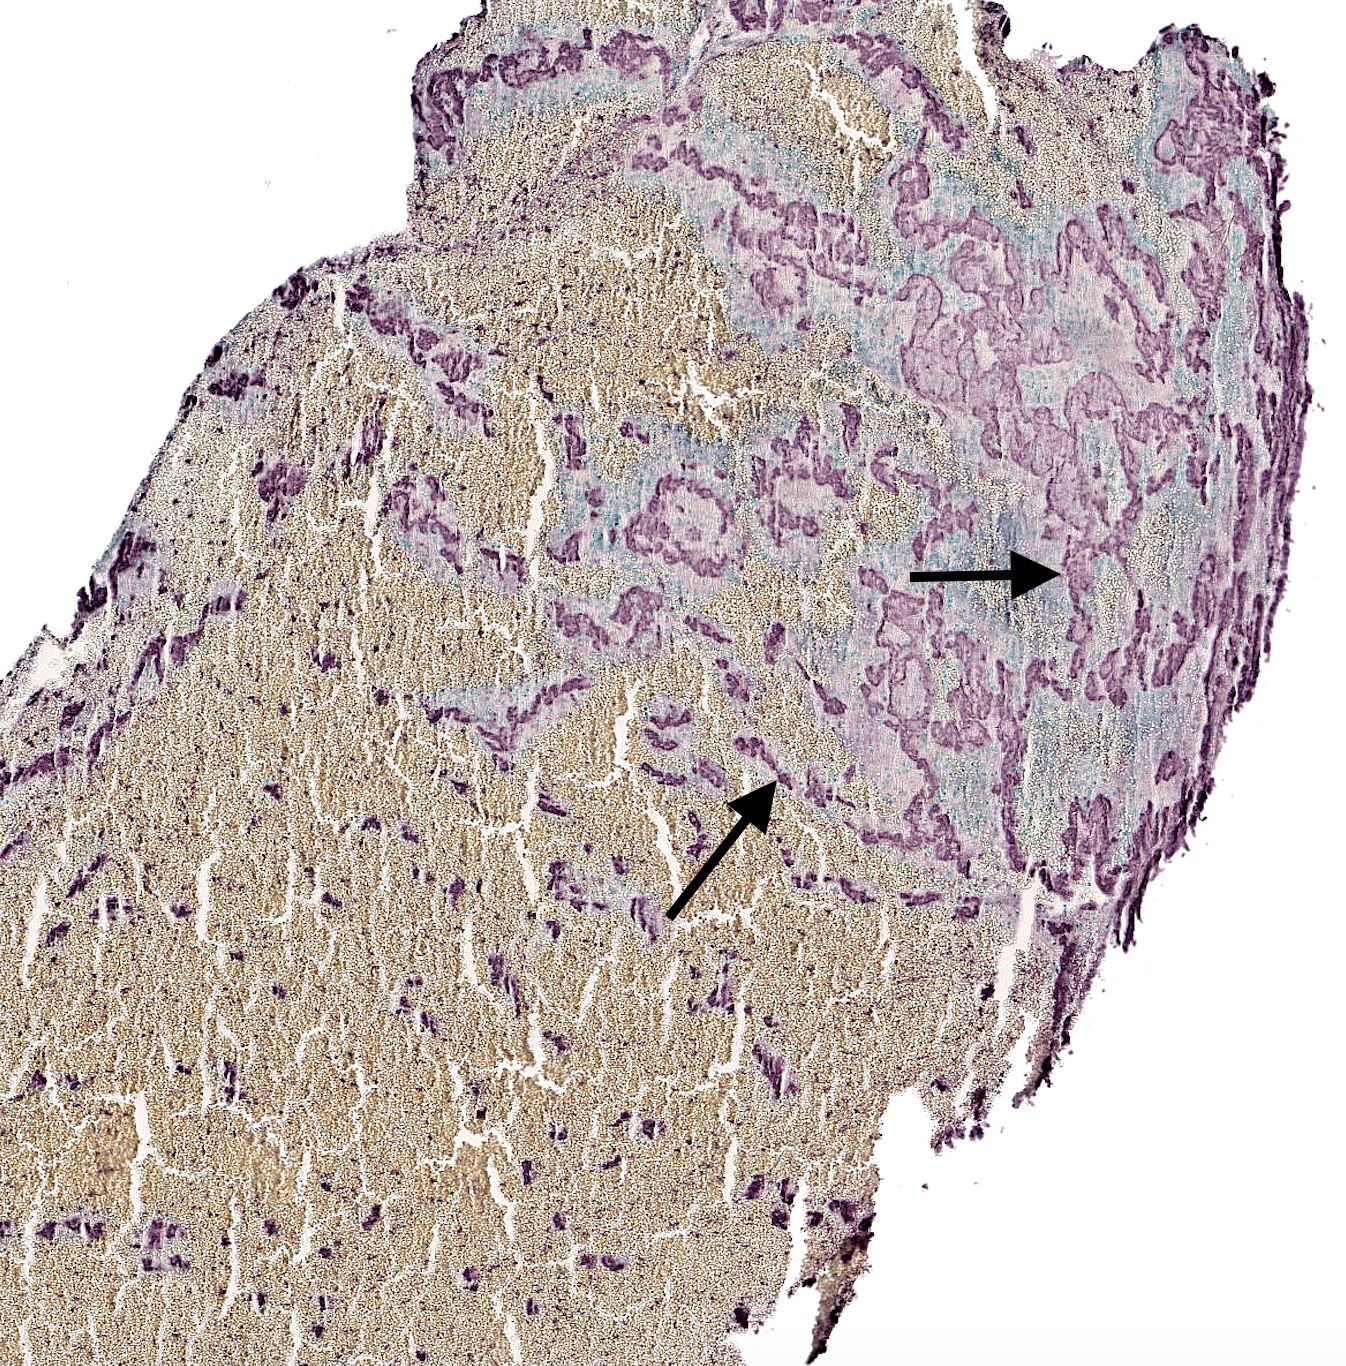
\includegraphics[width=7cm]{Indicator_vb1}}}
	\qquad
	\subfloat[]{{\includegraphics[width=7cm]{Indicator_vb2}}}
	
	\caption{Illustratie van de twee soorten indicator (respectievelijk paars en donkerroze) die gedetecteerd moeten worden. We zien duidelijk dat het detecteren op afbeelding (a) eenvoudiger zal zijn dan op afbeelding (b).}
	\label{figuur indicators}
\end{figure}

\section{Onze oplossing}
In dit hoofdstuk trachten we een oplossing te vinden voor ons probleem. We willen namelijk het percentage indicatorpixels in een willekeurige afbeelding kunnen berekenen. Het hoofdstuk is opgedeeld in verschillende deelproblemen: het verwijderen van de achtergrond, het lokaliseren van de indicator en de gebruiksvriendelijke app. Alle resultaten zijn bekomen met behulp van de programmeertaal MATLAB.

\subsection{Achtergrondverwijdering} \label{Achtergrondverwijdering}
Het eerste deelprobleem is het verwijderen van de achtergrond. Op de afbeeldingen is er heel wat vuiligheid te vinden. Voorbeelden hiervan zijn luchtbellen of kleine verkleuringen in de achtergrond zoals men ziet op de Figuur \ref{figuur achtergrondverwijdering}. Hieronder beschrijven we verschillende operaties om de grootste klonters te lokaliseren en alles wat geen klonter is uit de afbeelding te verwijderen. Dit leidt in feite tot een ruisvrije afbeelding.

\begin{figure}[H]
	\centering
	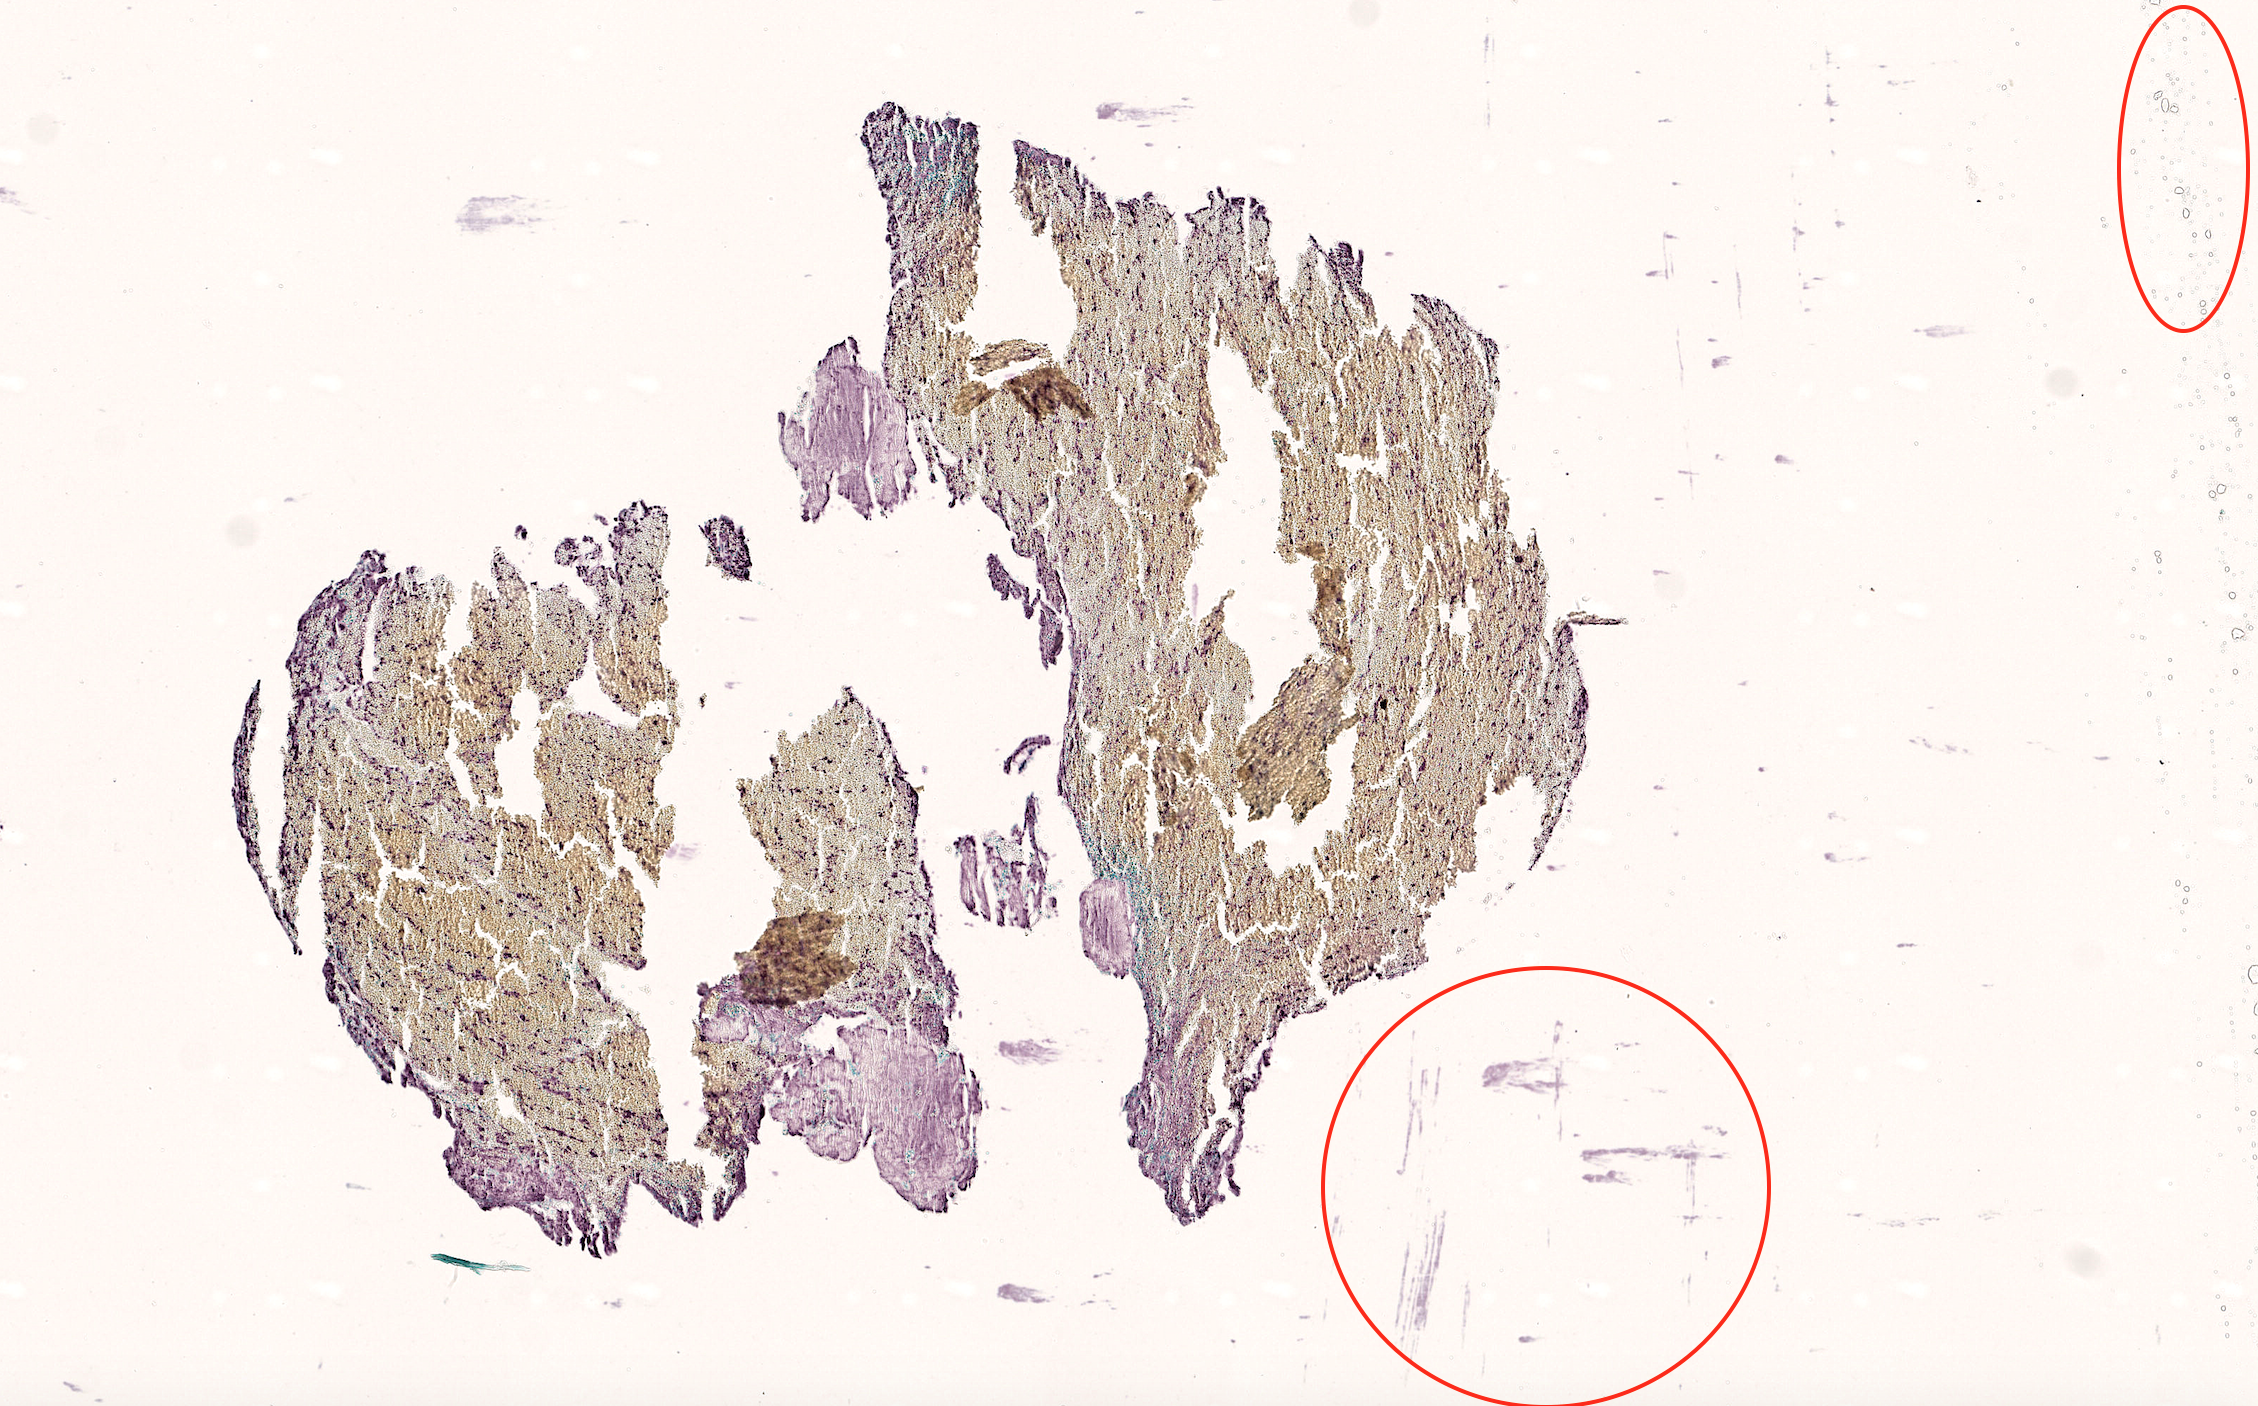
\includegraphics[width = 0.7\textwidth]{Ruis_afbeelding.png}	
	\caption{In de rechterbovenhoek zien we luchtbellen en in de onderste cirkel zien we een verkleuring die geen deel uitmaakt van een bloedklonter.}
	\label{figuur achtergrondverwijdering}
\end{figure}

\subsubsection{Bepalen van de beste threshold}
Het onderscheid tussen de achtergrond (eerder wit) en de bloedklonter (eerder grijs) is makkelijker te zien op de grijswaarden van de afbeelding, zie Figuur \ref{figuur beste_threshold}. Eén grijswaarde is nu voldoende om het onderscheid te maken. Een histogram van deze grijswaarden leert ons dat er een duidelijk dipje in de frequenties tussen het wit en het grijs te zien is, zie Figuur \ref{figuur graf1}. Dit is dan ook de theoretisch optimale threshold, de grijswaarde om een bloedklonterpixel van een achtergrondpixel te onderscheiden. Deze bepalen we simpelweg als het minimum in de tweede helft van de histogram. Wanneer we deze threshold toepassen, bekomen we de binaire Figuur \ref{figuur foto_bin}. Dit lijkt de klonters in de afbeelding nagenoeg goed te detecteren.

\begin{figure}[H]
	\centering
	\subfloat[]{{\includegraphics[width=6cm]{origineel_vb}}}
	\qquad
	\subfloat[]{{\includegraphics[width=6cm]{grijswaarden_vb}}}
	
	\caption{Illustratie van de originele foto (a) en deze omgezet in grijswaarden (b).}
	\label{figuur beste_threshold}
\end{figure}

\begin{figure}[H]
	\centering
	\includegraphics[width=0.85\textwidth]{GetBestthreshold_vb_aangeduid.png}
	
	\caption{Histogram van het aantal pixels gegroepeerd per grijswaarde. We zien duidelijk een lokaal minimum rond de waarde 230. Opmerking: we maken hier gebruik van een logaritmische y-as.}
	\label{figuur graf1}
\end{figure}

\begin{figure}[H]
	\centering
	\includegraphics[width=0.7\textwidth]{grijswaarden_bin_vb}
	\caption{Op deze binaire representatie zijn de bloedklonters duidelijk te zien.}
	\label{figuur foto_bin}
\end{figure}

\subsubsection{Ruisfilter}
Deze binaire representatie bevat heel wat holtes en ruis. In dit onderdeel proberen we dit probleem op te lossen. Hiervoor hebben we een simpele methode bedacht door enerzijds alle kleine groepen witte pixels te vervangen door zwarte pixels, zodat alleenstaande pixels (voornamelijk ruis) verdwijnen. Daarnaast vervangen we ook alle kleine groepen zwarte pixels door witte pixels, hierdoor worden daarenboven alle holtes in de bloedklonters opgevuld. Het resultaat van deze operatie is te zien op Figuur \ref{figuur ruisfilter} (a). \\
We bekomen nu een zogenaamde 'mask' die toegepast kan worden op de originele afbeelding. Hierbij worden alle zwarte pixels op de mask vervangen door witte pixels op de originele afbeelding. Alle witte pixels op de mask behouden hun kleur op de originele afbeelding. Daarnaast wordt deze afbeelding nog bijgesneden om kostbare geheugenruimte te sparen, de afbeelding is te zien is in Figuur \ref{figuur ruisfilter} (b). In dit deelprobleem werd echter met een reeds bijgesneden bloedklonter gewerkt om de afbeeldingen duidelijk te houden. Een volledig onbewerkte afbeelding is echter te zien in Figuur \ref{figuur volledig_onbewerkt}

\begin{figure}[H]
	\centering
	\subfloat[]{{\includegraphics[width=7cm]{ruisvrij_vb}}}
	\qquad
	\subfloat[]{{\includegraphics[width=7cm]{ruisvrij_kleur_vb}}}
	
	\caption{Alle ruis is verwijderd, dit is een foto die verder verwerkt kan worden.}
	\label{figuur ruisfilter}
\end{figure}

\begin{figure}[H]
	\centering
	\includegraphics[width=15.25cm]{Volledig_onbewerkt}
	
	\caption{Dit is een volledig onbewerkte afbeelding die we in \ref{figuur ruisfilter} (b) hebben bijgesneden en waarvan de achtergrond verwijderd is.}
	\label{figuur volledig_onbewerkt}
\end{figure}

\subsubsection{Uitzonderingen}
Naast de gewone bloedklonters zijn er ook nog enkele uitzonderingen. Sommige klonters hebben namelijk geen rode bloedcellen waardoor ze zeer wit zijn. Dit zien we ook op Figuur \ref{figuur lichte_kleuring}. Het probleem is dat we hier geen optimale threshold kunnen berekenen zoals eerder uitgelegd. Er is namelijk een zeer kleine afstand tussen de kleur van de bloedklonter en de feitelijke achtergrond. Vandaar dat we in de app een slider verwerkt hebben om desnoods zelf die threshold aan te aanduiden. Wanneer de optimalisaties van de simpele binaire mask daarna op deze threshold toegepassen, bekomen we Figuur \ref{figuur lichte_kleuring_binair}. Het is duidelijk te zien dat dit algoritme zeer krachtig is in het detecteren van bloedklonters.

\begin{figure}[H]
	\centering
	\includegraphics[width=0.7\textwidth]{lichte_kleuring}
	
	\caption{Een afbeelding van een bloedklonter zonder rode bloedcellen.}
	\label{figuur lichte_kleuring}
\end{figure}

\begin{figure}[H]
	\centering
	\includegraphics[width=0.7\textwidth]{lichte_kleuring_binair}
	
	\caption{Dit is de binaire mask die we bekomen na het toepassen van de threshold en de optimalisatie van deze. De klonters worden nu met zekere precisie aangeduid.}
	\label{figuur lichte_kleuring_binair}
\end{figure}


\subsection{Lokalisatie van de indicator} \label{lokalisatie_indicator}
Het tweede deel van ons project is de indicators lokaliseren en kwantificeren. Ons project moet in staat zijn twee specifieke soorten van indicatoren te onderscheiden. Van deze is een voorbeeld op Figuur \ref{figuur indicators} te zien. Omdat het kleurverschil tussen wat aangeduid worden (indicator) en wat niet (achtergrond) niet altijd even groot is, vormen we het oorspronkelijke \textit{RGB} kleurmodel\footnote{Het RGB kleurmodel is een voorstelling waarbij ieder kleur voorgesteld wordt door een waarde van de drie basiskleuren (rood, groen en blauw)} om naar het zogenaamde \textit{HSV} kleurmodel. Dit model is een alternatieve voorstelling waarbij men alle kleuren op een cirkel voorstelt, de hoek die dit kleur dan maakt, noemt men de \textit{Hue}. Naast deze waarde heeft \textit{HSV} nog twee andere parameters namelijk \textit{Saturation} en \textit{Value}. \textit{Saturation} kan simpel beschouwd worden als een aanduiding van de hoeveelheid witte kleur en \textit{Value} een aanduiding van de zwarte kleur. Een grafische voorstelling is te zien op Figuur \ref{figuur hsv_schema}.\\
Het voordeel van deze transformatie is dat het heel wat eenvoudiger is om een onderscheid tussen dichtbijgelegen kleuren te vinden. Een andere mogelijke transformatie is die naar het \textit{LAB} of het \textit{CMYK} kleurmodel die gelijkaardige eigenschappen heeft en desnoods ook gebruikt kan worden. Eenmaal we een duidelijk onderscheid tussen de indicator en de achtergrond gemaakt hebben, berekenen we eenvoudig het percentage indicator als de verhouden van het aantal bloedklonter- en indicatorpixels. Ons stappenplan wordt in de volgende hoofdstukken besproken en wordt toegepast op de afbeelding uit Figuur \ref{figuur indicators} (a). Maar kan evenwel gebruikt worden op de andere kleuring met andere beginwaarden.

\begin{figure}[H]
	\centering
	\includegraphics[width=0.7\textwidth]{HSV_vb.png}
	
	\caption{Grafische voorstelling van het \textit{HSV} (\textit{Hue}, \textit{Saturation}, \textit{Value}) kleurmodel}
	\label{figuur hsv_schema}
\end{figure}

\subsubsection{Het HSV kleurmodel}
Zoals reeds vermeld, beginnen we met een transformatie naar het \textit{HSV} kleurmodel. Bijgevolg kunnen we de twee voorstellingen vergelijken. We hebben het model telkens ontbonden in de drie kleurwaarden, waarbij zwart de laagste waarde voor dat kleur voorstelt en wit de hoogste. De resultaten zijn te zien in de Figuren \ref{figuur RGB} en \ref{figuur HSV}. Het verschil tussen de twee kleurmodellen is duidelijk te zien. Afbeelding (a) en (b) uit Figuur \ref{figuur HSV} lijken namelijk een iets agressiever onderscheid te maken.

\begin{figure}[H]
	\centering
	\subfloat[]{{\includegraphics[width=4.5cm]{RGB_r}}}
	\qquad
	\subfloat[]{{\includegraphics[width=4.5cm]{RGB_g}}}
	\qquad
	\subfloat[]{{\includegraphics[width=4.5cm]{RGB_b}}}
	\caption{Illustratie van respectievelijk de rode, groene en blauwe kleurwaarden (\textit{RGB}). Hierbij komt wit overeen met de maximumwaarde en zwart met de minimumwaarde van die kleur.}
	\label{figuur RGB}
\end{figure}

\begin{figure}[H]
	\centering
	\subfloat[]{{\includegraphics[width=4.5cm]{HSV_h}}}
	\qquad
	\subfloat[]{{\includegraphics[width=4.5cm]{HSV_s}}}
	\qquad
	\subfloat[]{{\includegraphics[width=4.5cm]{HSV_v}}}
	
	\caption{Illustratie van respectievelijk de \textit{hue}, \textit{saturation} en \textit{value} kleurwaarden (\textit{HSV}). Hierbij komt wit overeen met de maximumwaarde en zwart met de minimumwaarde van die kleurwaarde.}
	\label{figuur HSV}
\end{figure}

\subsubsection{Een algemene threshold}
De volgende stap is een filter bepalen voor de indicatorpixels. Het probleem is echter dat een goede filter voor de ene afbeelding niet altijd een goede filter voor de andere is. Daarom hebben we voor iedere afbeelding afzonderlijk manueel een 'threshold' bepaald en deze achteraf met elkaar vergeleken. Het resultaat is bijgevolg een vrij algemene threshold die alle indicatorpixels met zekerheid aanduidt, zoals te zien is op Figuur \ref{figuur alg_tresh}. Het enigste probleem is dat bepaalde pixels verkeerd aangeduid worden. Het aantal is weliswaar niet zo groot, maar aangezien ze in iedere afbeelding voorkomen zullen we dit trachten te omzeilen.
\begin{figure}[H]
	\centering
	\includegraphics[width = 0.7\textwidth]{algemene_threshold}
	
	\caption{We hebben alle indicatoren met een blauwe kleur aangeduid. De algemene threshold selecteert alle indicatorpixels, maar jammer genoeg ook enkele verkeerde, deze zijn aangeduid met een pijl.}
	\label{figuur alg_tresh}
\end{figure}

\subsubsection{Optimalisatie van de threshold} \label{additional_filter}
In dit hoofdstuk willen we het aantal verkeerde pixels verminderen zonder de juiste te beïnvloeden. We hebben echter al een vrij correcte threshold waardoor we een statistische analyse van wat onder de bijhorende mask ligt, kunnen uitvoeren. Hiervoor stellen we een histogram van de \textit{HSV} kleurwaarden onder de mask op. Het levert ons een interessant resultaat dat te zien is in Figuur  \ref{figuur HSVHIST}. We zien namelijk duidelijke verschillen in de frequenties van bepaalde kleurwaarden.\\
Het idee is om nu de verkeerde pixels via deze diagrammen eruit te filteren. Hiervoor doen we de aanname dat de verkeerde pixels essentieel in kleur verschillen van indicatorpixels. We weten ook uit Figuur \ref{figuur alg_tresh} dat verkeerde pixels minder vaak voorkomen dan de juiste. De huidige threshold zou dus in feite manueel bijgestuurd kunnen worden, maar dit heeft geen zin. De grafieken van verschillende afbeelding hebben namelijk eenzelfde vorm, maar hun pieken liggen soms meer dan 5\% verschoven. Daarom passen we op iedere afbeelding afzonderlijk automatisch een filter toe. In principe kunnen alle pixels met een frequentie onder een bepaalde grenswaarde geschrapt worden. Maar een betere benadering is misschien om het punt te vinden, waar de frequentie van de pixels enorm begint toe te nemen. Indien we deze thresholdwaarde naar de pieken toeschuiven, zijn we eigenlijk grote 'indicatoraders' aan het verwijderen. Dit zien we op Figuur \ref{figuur HSVHIST_aangeduid}. Dit punt kan theoretisch benaderd worden als het maximum van de tweede afgeleide naar de kleurwaarde. \\
Wanneer we deze filter toepassen, bekomen we het resultaat dat te zien is op Figuur \ref{figuur morf} (a). De zones die eerder verkeerd werden aangeduid zijn nu bijna volledig verdwenen.\\
Een extra stap die we tenslotte nog toepassen is het morfologisch sluiten van de pixels. Dit doen we door indicatorpixels die niet ver van elkaar gelegen zijn met elkaar te verbinden. Het is namelijk zo dat wanneer een pixel omringt is door indicatorpixels, de kans hoog is dat deze pixel ook een indicatorpixel is. Het resultaat is te zien op \ref{figuur morf} (b).\\
De laatste stap die nu nog rest is het optellen van alle aangeduide pixels en de bloedklonterpixels. Wanneer we dan de verhouding nemen, bekomen we het percentage indicator, wat net gevraagd werd.


\begin{figure}[H]
	\centering
	\subfloat[]{{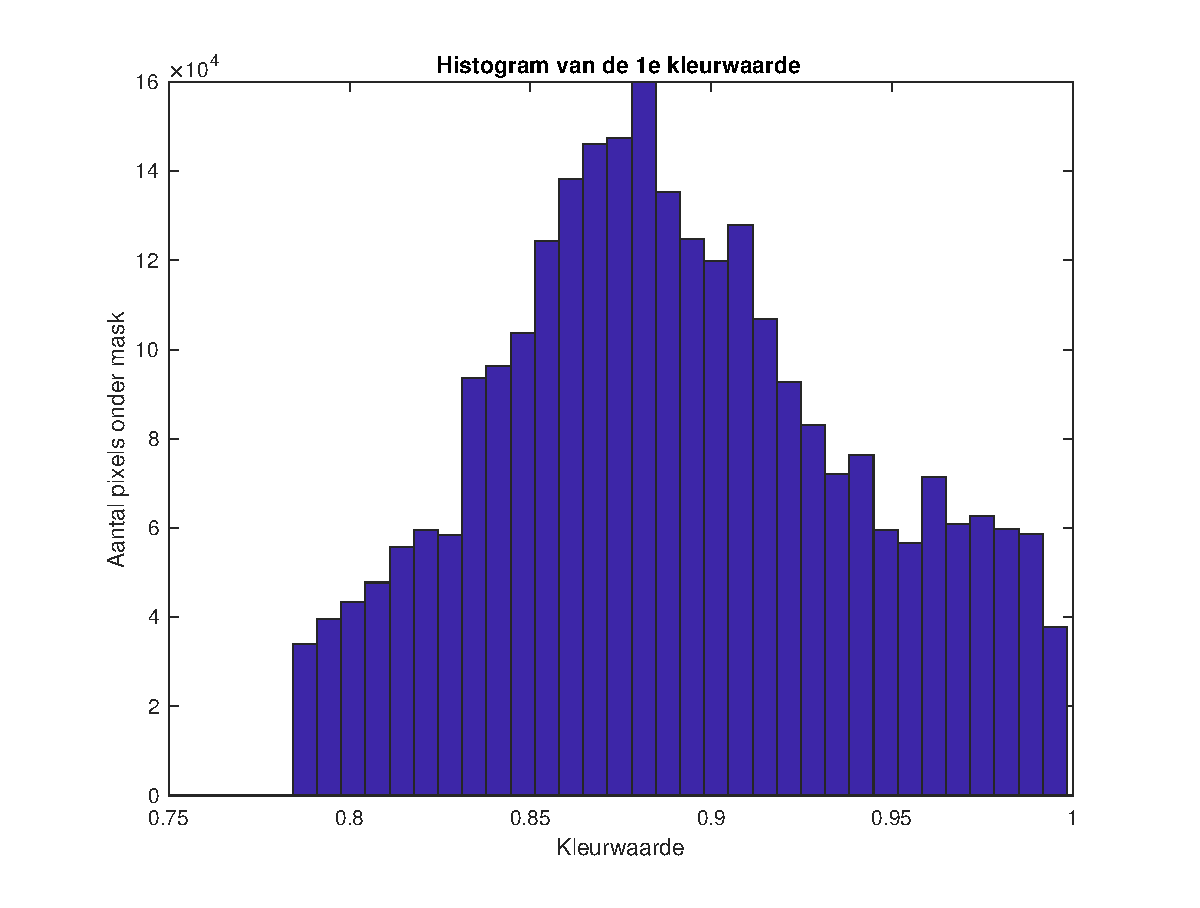
\includegraphics[width=4.5cm]{hsvhist_h}}}
	\qquad
	\subfloat[]{{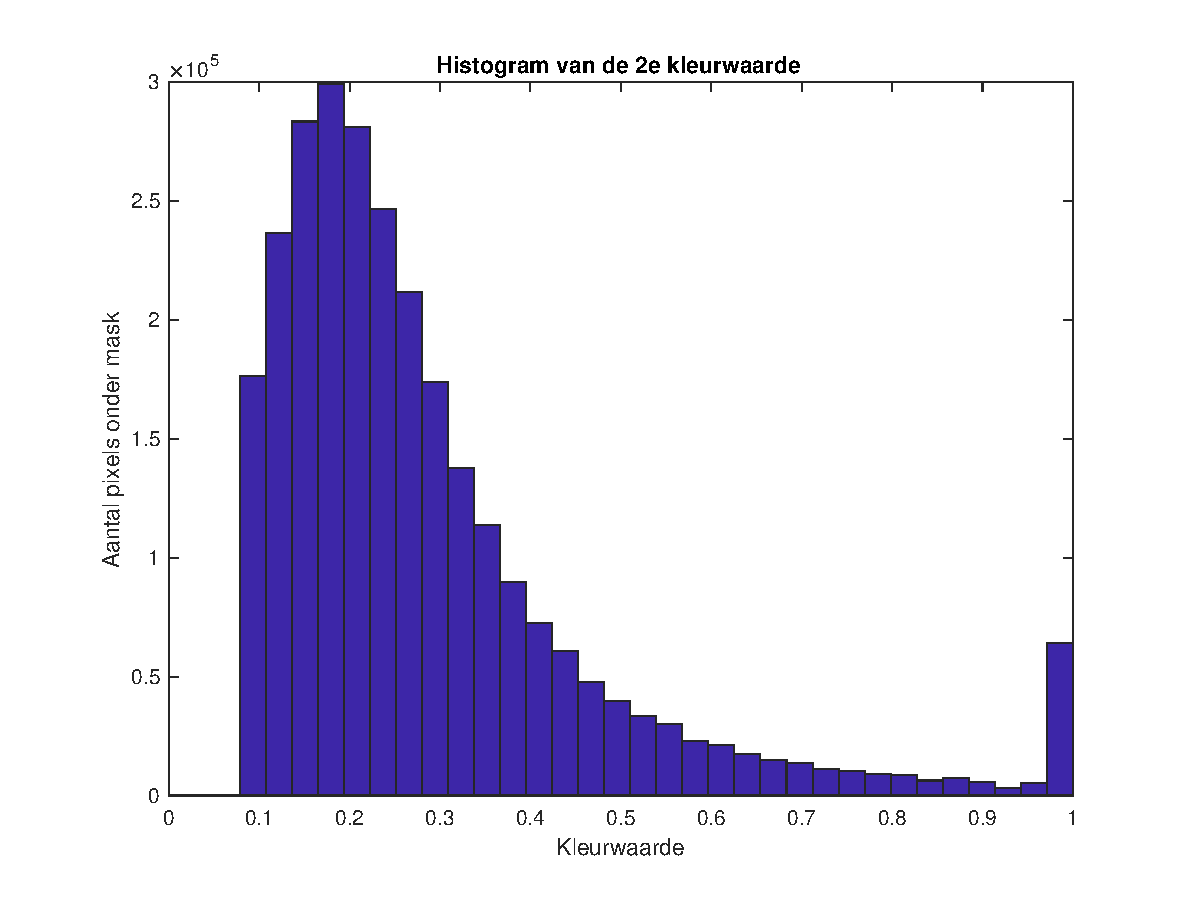
\includegraphics[width=4.5cm]{hsvhist_s}}}
	\qquad
	\subfloat[]{{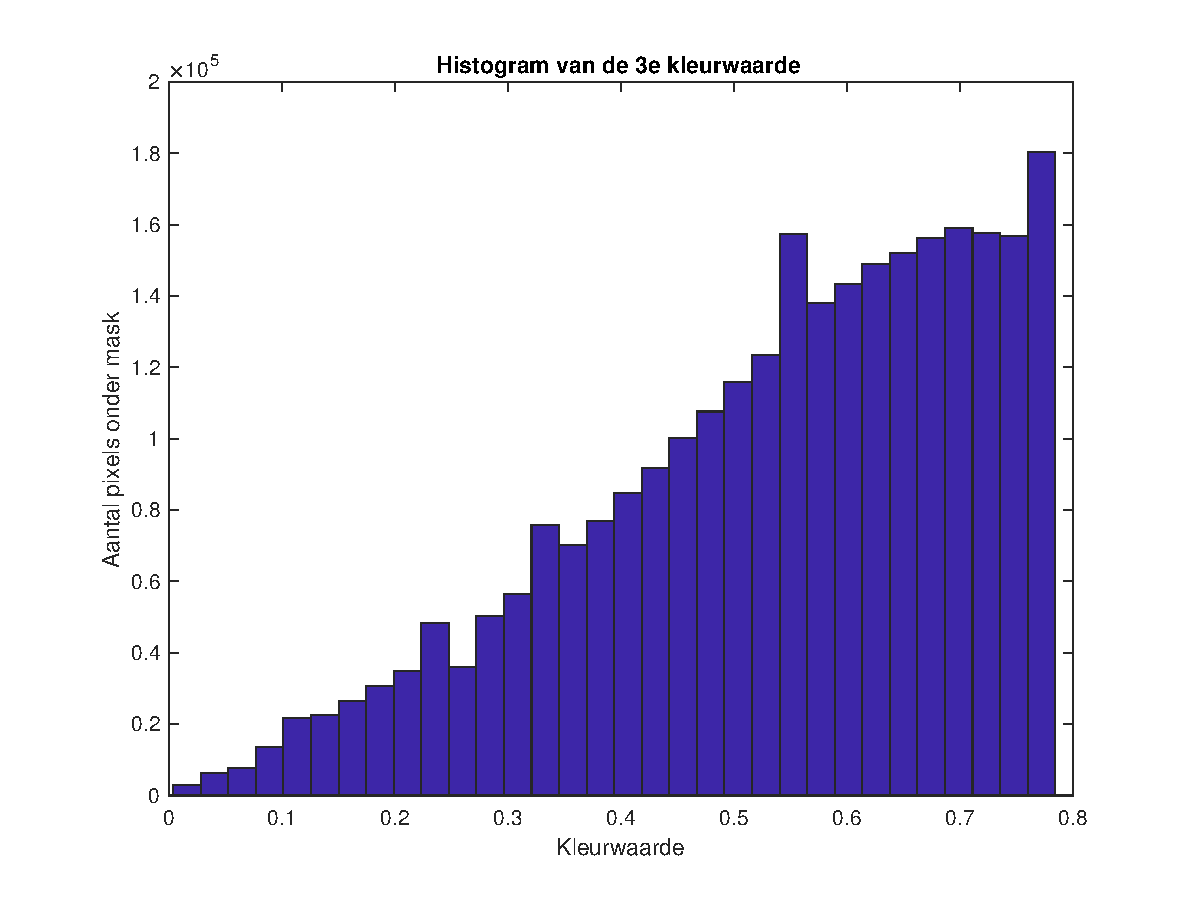
\includegraphics[width=4.5cm]{hsvhist_v}}}
	
	\caption{Histogrammen van de HSV kleurwaarden. We zien duidelijk het verschil in frequenties.}
	\label{figuur HSVHIST}
\end{figure}

\begin{figure}[H]
	\centering
	\subfloat[]{{\includegraphics[width=0.7\textwidth]{hsvhist_aangeduid}}}
	
	\caption{Op de figuur is hebben we een punt op de curve aangeduid. Wanneer we dit punt naar links verschuiven, verwijderen we telkens grotere stukken indicator van onze afbeelding. Dit willen we net vermijden.}
	\label{figuur HSVHIST_aangeduid}
\end{figure}

\begin{figure}[H]
	\centering
	\subfloat[]{{\includegraphics[width=7cm]{threshold_filtered}}}
	\qquad
	\subfloat[]{{\includegraphics[width=7cm]{threshold_morfologisch}}}
	
	\caption{Illustratie waarbij we in (a) een algoritmische filter hebben toegepast om mogelijke ruis te verwijderen. De pijltjes zijn de zones die weggefilterd zijn op Figuur \ref{figuur alg_tresh}. In afbeelding (b) hebben we deze mask nog eens morfologisch gesloten, waardoor we een duidelijke aanduiding van de indicatorpixels bekomen.}
	\label{figuur morf}
\end{figure}

\subsubsection{Problemen}
We kunnen nu wel met redelijke precisie de indicatoren in de afbeelding aanduiden, maar dit is niet even simpel voor iedere afbeelding.
Het probleem met deze kleuringen is namelijk dat er heel wat variatie in de afbeeldingen zit. De effectieve kleuring in het labo is afhankelijk van verschillende factoren zoals bijvoorbeeld temperatuur, druk, luchtvochtigheid... Hierdoor kan deze kleuring van dag tot dag in intensiteit verschillen. Daarenboven zijn wij als student ingenieurswetenschappen ook niet getraind om rode bloedcellen te detecteren. Bijgevolg hebben we in onze app ervoor gezorgd dat onze filter met behulp van verschillende sliders altijd bijgestuurd kan worden door de gebruiker en dus toch het gewenste resultaat bekomen kan worden.


\subsection{De gebruiksvriendelijke applicatie}
Naast het verwerken van de klonters is het ook de bedoeling dat de afbeelding op een makkelijke manier verwerkt kan worden. Vandaar dat we een gebruiksvriendelijke app in MATLAB ontwerpt hebben.
Een screenshot van de grafische interface is te zien op Figuur \ref{figuur interface}. In dit hoofdstuk zullen we kort de functionaliteiten van deze app beschrijven.\\
De app kan op twee verschillende manieren gebruikt worden. In eerste instantie kan men een afbeelding ingeven die dan uiteindelijk het volledige verwerkingsproces van hoofdstuk \ref{Achtergrondverwijdering} en \ref{lokalisatie_indicator} doorloopt. Men begint met een afbeelding en een folder om de tussenresultaten op te slaan te kiezen. In de eerste fase van het verwerkingsproces wordt de afbeelding bijgesneden zodat enkel de bloedklonter nog zichtbaar is. Deze bijgesneden afbeelding wordt dan getoond. Indien men niet blij is met de bekomen resultaten kan men manueel de threshold bijsturen. Vervolgens begint de kleurenanalyse, hier wordt de volledige afbeelding verwerkt om uiteindelijk een percentage indicator aan te duiden. Deze verwerkte afbeelding wordt dan ook getoond zoals te zien is op Figuur \ref{figuur interface}. Daarnaast wordt het percentage van de hoeveelheid aanwezige indicator weergegeven. Indien men niet tevreden is met het resultaat, kan men een transformatie naar een andere kleurruimte (HSV, CMYK of RGB) toepassen. Daarnaast kan men ook met verscheidene sliders een manuele selectie van de indicator doen. Men kan ten slotte nog opteren om de additionele filter uit hoofdstuk \ref{additional_filter} uit te schakelen. \\
De app kan ook op een nog andere manier gebruikt worden. Men kan namelijk een volledige folder met afbeeldingen selecteren om de achtergrond van iedere afbeelding te verwijderen. Deze afbeeldingen worden bijgevolg opgeslagen in een eerder gedefinieerde folder.

\begin{figure}[H]
	\centering
	\subfloat[]{{\includegraphics[width=\textwidth]{interface_app}}}
	
	\caption{Afbeelding van de grafische interface van de app.}
	\label{figuur interface}
\end{figure}


\section*{Besluit}



\includepdf[pages={1-3}]{ganttchart}

\end{document}
